\documentclass{article}

\usepackage{neurips_2020_author_response}

\usepackage[utf8]{inputenc} % allow utf-8 input
\usepackage[T1]{fontenc}    % use 8-bit T1 fonts
\usepackage{hyperref}       % hyperlinks
\usepackage{url}            % simple URL typesetting
\usepackage{booktabs}       % professional-quality tables
\usepackage{amsfonts}       % blackboard math symbols
\usepackage{nicefrac}       % compact symbols for 1/2, etc.
\usepackage{microtype}      % microtypography
\usepackage{subcaption}
\usepackage{graphicx}
\usepackage{wrapfig}

\begin{document}

First, thank all the referees for offering valuable suggestions to help improving the writting of the paper.
The referees generally agree that our paper is innovative in some aspects, but needs some improvement in the writting.
We will definitely improve our writting before cameraready.
\textbf{The authors feel depressed that 2/4 referees think our result can not be reproduced. Although both NiLang and the benchmarks are open source on Github.}

Some referees think our work lack of comparison to strong baseline like Tensorflow and Pytorch.
This is not true, Tapenade is a very strong baseline in the field of \textbf{generic} AD.
%The meaning of automatic differentiation has been changed dramatically recent years,
%i.e. many people view Tensorflow and Pytorch as automatic differentiation package now.
%The classical automatic differentiation only concerns source code level differentiations,
%the most important feature is we need only a limited number of low level instructions to differentiate an arbituary program.
%To avoid confusion, I call the general purposed traditional AD the programing language automatic differentiation (PL-AD).
Tensorflow and Pytorch are \textbf{domain specific} AD softwares for traditional tensor based machine learning.
%Since both Tensorflow and Pytorch are very solid packages and both are backended by CuBLAS. No one can beat them in their own domain of tensors, hence there is no need for yet another tensor based AD tool.
There are applications that not suited for tensors.
e.g. People benchmarked Tensorflow, Pytorch and Tapenade in the bundle adjustment application as shown in the figure.

\begin{wrapfigure}{l}{0.5\textwidth}
    \centerline{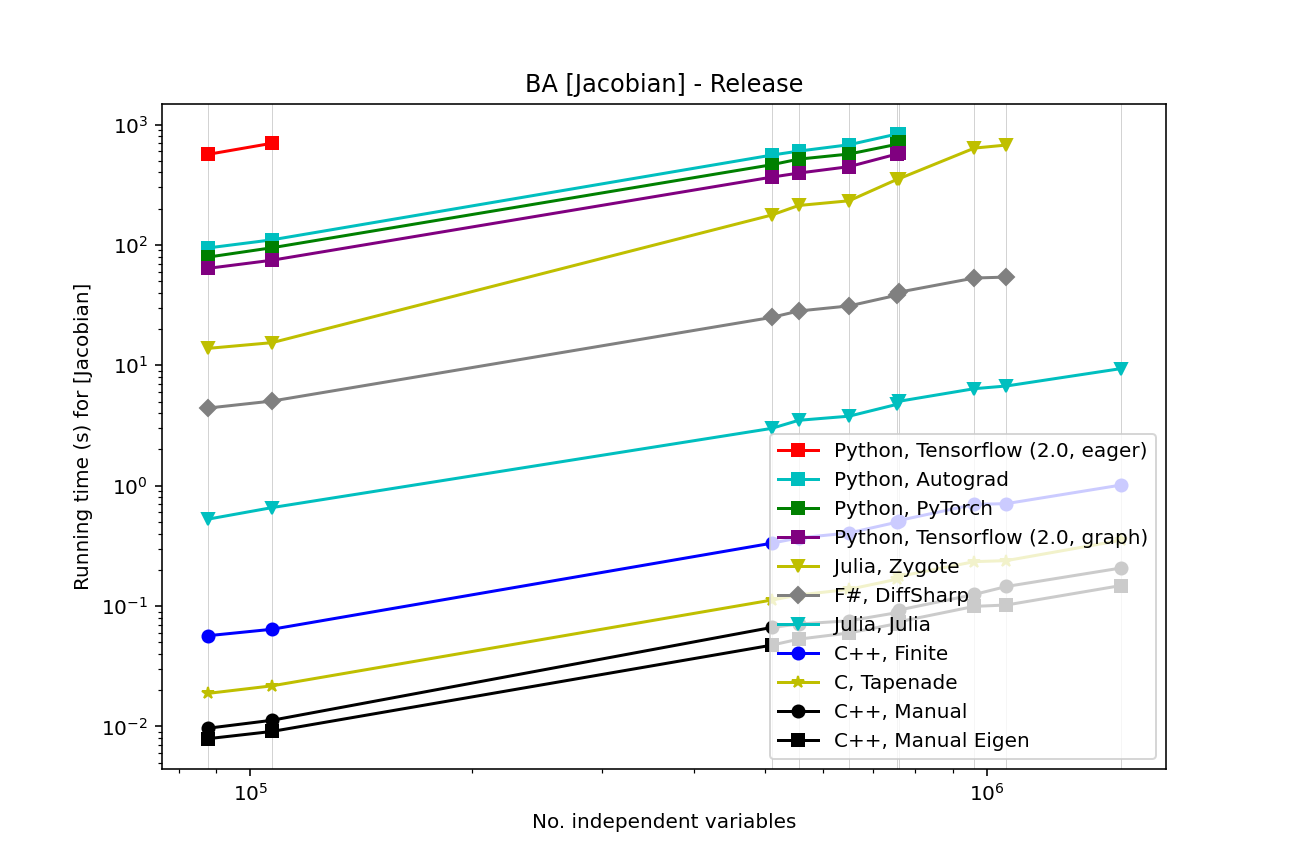
\includegraphics[width=0.5\columnwidth,trim={0 0cm 0 0cm},clip]{ba-jacobian-adbench.png}}
    \caption{The bundle adjustment benchmark which includes Pytorch and Tensorflow (conducted by the ADBench project of microsoft).}\label{bench-ba}
\end{wrapfigure}

Tapenade is $10^{3-5}$ times faster than Pytorch and Tensorflow. However Tapenade is commercial, close sourced and C/Fortran based.
I am pround that NiLang is even better than Tapenade in this benchmark.
I strongly recommend refereees to read the ADBench paper [arXiv:1807.10129], you will be supprise that we choose one of the worlds' best generic AD package as our benchmark target.
We don't benchmark the popular Julia package Flux because it is backended on Zygote, we benchmarked Zygote instead. NiLang is more than one order faster than Zygote in the graph embedding benchmark.
%After all, I want to emphasis, benchmarking with Tensorflow and Pytorch on the generic AD is not fair, because they are domain specific.

Some referees are wondering if reversible computing are some kind equivalent to tranditonal AD with optimized checkpointing.
I want to emphsis that reversible programming shows advantage in speed and memory comparing with traditional generic AD for one simple reason: \textit{the coding style and reversible thinking matters.}
In NiLang, a programmer does not have the chance to write ``bad'' code just because every allocation is explicit.
In the sparse matrix dot product example in the appendix.
A reversible program has to preallocate a \texttt{branch\_keeper} to store the decisions of branches to enforce reversibility inside the loop.
If a user is writting it in a freestyle, it impossible to avoid stack operations inside the loop, which will slow down the program.
Allocate automatically for a user is even more dangerous in GPU programming.
In the bundle adjustment benchmark, %if the AD compiler insert stack operations in the AD code without informing a user,
%the code will break unexpectedly when compiled to the GPU. In NiLang, 
we can compile the code on GPU to enjoy a ~200x speed up with no more than 10 extra lines of code.
It is very easy for users to completely avoid allocation inside a loop in NiLang.
On the other side, the optimal checkpointing is a well known hard problem. It does not support using reversibility naturally, and a user does not have full control of the allocation.

One of the referee is interested to know the limitations of NiLang. We don't think there will be a differentiable program that can not be not be written reversiblly because any program can be made reversible by storing the inputs. The most severe weakness of NiLang is the floating point arithmetic used for computing suffers from the rounding error.
This issue has a systematic solution by mixing fixed point number and logarithmic number, which will be explain in the next update.
%One of the referee mention that to handle the backward rule of ``+'' operation, one do not need to store the inputs of an instruction, gradient of both inputs are $1$. There is no need to trace back the state. This is true. In our current version, we haven't put effort in optimizing such operations yet.
%In NiLang, the backward propagation program generally contains $\sim2$ times more instructions than the forward pass. This factor is estimated by considering the backward rule of the multiplication operation. This is a known bottleneck in the field of generic AD.

%A referee mentions that SVD is available in Tensorflow and Pytorch, this is true.
%I have cited the some recent developments in the main text, including arXiv 1909.02659. One of the author of this paper submitted the PR \#32226 of complex valued SVD to tensorflow.
%However, in the main text, what I want to emphasis is that the backward rules are manually derived, and can be quite complicated to derive the backward rules for some functions.
%Sorry for the confusing statements in the main text.
%I also agree that I should cite the serie of papers in machine learning field that utilize reversibility, including i-RevNet, unitary RNN, residual network with reversible activation functions and normalizing flow,
%that should be a good supporting materials that how reversibility can be useful in reducing the memory usage.
%I have been tracking these papers for a long time, it is a huge mistake for not including them in the reviewed version.
%For the comparison between checkpointing, they are available at the end of the supplimentary material. They should be moved to the main text.
%Checkpointing is a part of reversible computing. In reversible computing, checkpointing is an equivalent to the cascade layout of adibatic CMOS, the more integrable layout is the pipeline layout that utilize reversibility. The problem of checkpointing is it does not utilies reversibility in a straight foward way, many BLAS function are purely composed of reversible function, there is no need to checkpoint at all. Any arithematic function computed with Taylor expansion can be computed in constant memory by combining fixed point number system and logarithmic number system, which will be explained in detail in the next update.
%The use the reversible $\mathrel{*}=$ operation in logarithmic numbers in Taylor expansion is nessesary to avoid cahing intermediate data. Which is another win of reversible thinking.

%because checkpointing itself is a naive strategy to achieve reversibility. I think the referee wants the emphasis whether there are reversible applications that can not be written reversiblly without extra memory overhead
%An important class of application that must include caching inside a for loop is the integrator
%Although an integrator ``looks'' reversible, most integrators are not truely reversible, their reversible implementation has no advantage comparing with optimal checkpointing
%One expception is the time reversible leapfrog integrator for solving symmpletic system.

Some referees want to know from which aspect NiLang is different from a traditional reversible programming language.
For a long time, the reversible programming languages concerns too much about theoretical elegance and ignored the productivity.
NiLang is special for that it supports many practical elements like arrays, complex numbers, fixed point numbers and logarithmic numbers and is being an eDSL so that it can be used directly to accelerate Zygote framework in Julia.
%NiLang is a very good fit with Julia, because Julia is a ideal platform for scientific programming.
%I think NiLang is special, just because it conveys information that even in the irreversible software stack, we gain a lot by utilizing reversible programming.
%NiLang is an important step to get our software stack ready for future hardwares.

At last, I wish referees can evaluate this project more from the ``furture'' perspective.
Nowadays, the energy is becoming one of the most deadly bottleneck for machine learning applications.
As a quantum physicist, I believe that reversible computing is the only correct approach to solve the energy conundrum.
Classical reversible computing has been scilented for $\sim$15 years, NiLang is trying to bridge machine learning and the reversible computing.
We will try our best to convey this point better in the updated version.

I will address other comments like SVD is available in Pytorch and Tensorflow,
comparing reversible programming and the use of reversibility in ML in the main text directly. Thanks for your valuable information.


%Unlike quantum computing, classical reversible technology like adiabatic CMOS are very close to us.
%Within 5-10 years, there should be reversible hardwares that can decrease the dynamic energy dissipation of traditional CMOS by an order of $\sim$2 (according to the numeric simulation). It should be an idea platform that our NiLang can be compiled to.

%Reversible computing is a ``dead'' field in the last 15 years. It faces strange dilema that
%\begin{itemize}
%    \item Reversible computing uses a completely different software stack, and is know to have a lot overhead in the software level, if there is no good software stack, there will be no hardware.
%    \item If there is no reversible hardware to save energy, there will be no reversible software stack.
%\end{itemize}

\end{document}
